\documentclass[../ecuaciones_diferenciales.tex]{subfiles}

\begin{document}

Las ecuaciones diferenciales son ecuaciones que relacionan una o varias
funciones con sus derivadas, de forma que la incógnita es una función o tupla de
funciones que cumpla dicha relación. Como puede imaginarse, estas ecuaciones
serán muy útiles en cualquier contexto en el que se conozca cómo influye el
valor de una función a su tasa de crecimiento o viceversa.

En este curso nos centraremos exclusivamente en el estudio de las ecuaciones
diferenciales ordinarias (EDO), que son ecuaciones diferenciales que contienen
una o varias funciones en una sola variable (normalmente el tiempo). Más
generalmente, las funciones pueden depender de más de una variable, pero las
derivadas se hacen únicamente respecto a una de ellas; de esta forma, el resto
de variables se pueden considerar como parámetros. En particular, estudiaremos
casi exclusivamente las ecuaciones diferenciales ordinarias \emph{lineales}, por
su sencillez.

El término \textquote{ecuación diferencial ordinaria} se usa en contraposición
al de \textquote{ecuación en derivadas parciales} (EDP), una ecuación
diferencial en la que aparecen funciones en varias variables y derivadas
parciales respecto a más de una de ellas.

Veremos que muchos fenómenos físicos pueden ser modelados mediante ecuaciones
diferenciales y aunque las más interesantes, como las que modelan la dinámica de
fluidos (ecuaciones de Navier-Stokes) o la propagación del calor en una región
(ecuación del calor), son ecuaciones en derivadas parciales, muchos fenómenos
pueden ser modelados con ecuaciones diferenciales ordinarias. Históricamente,
las ecuaciones diferenciales surgieron de la mano de la física y así ha seguido
hasta principios del siglo XX; incluso a día de hoy, encuentran aplicaciones de
forma muy natural en el campo de la física porque la mayoría de las leyes en
esta disciplina están formuladas matemáticamente. No obstante, también tienen
usos muy importantes en campos como la ecología, la economía e incluso la
medicina, algunos de los cuales analizaremos aquí.

Antes de abordar estas cuestiones en detalle necesitamos introducir algunas
definiciones.

\section{Primeras definiciones}

\begin{definition}[Ecuación diferencial]
	Una ecuación diferencial es una ecuación de la forma
	\[F(t, x, x', x'', \dots, x^{(n)}) = 0\]
	donde \(F : \Omega \to \R\) con \(\Omega \subset \R^{n + 2}\) abierto.
\end{definition}

\begin{definition}
	Se dice que \(x(t)\) es solución de una ecuación diferencial en el intervalo
	\(I \subset \R\) si \(x : I \to \R\) y
	\[F(t, x(t), x'(t), x''(t), \dots, x^{(n)}(t)) = 0, \quad \forall t \in I.\]
	Se cumple además que:
	\begin{enumerate}[i)]
		\item La función \(x\) tiene todas las derivadas hasta orden \(n\) y son
		      continuas.

		\item El punto \((t, x(t), x'(t), \dots, x^{(n)}(t)) \in \Omega\) para
		      todo \(t\) en \(I\).
	\end{enumerate}
\end{definition}

Supondremos que la ecuación diferencial está dada en forma normal.

\begin{definition}[Forma normal]
	Una ecuación diferencial está escrita en forma normal si es una expresión 
	de la forma
	\begin{equation} \label{eq:forma_normal}
		x^{(n)} = f(t, x', x'', \dots, x^{(n - 1)})
	\end{equation}
\end{definition}

Llamaremos \(\Omega \subset \R^{n + 1}\) al dominio de \(f\), esto se puede 
hacer localmente sin pérdida de generalidad gracias al teorema de la función
implícita.

\begin{definition}[Orden]
	Llamaremos orden de la ecuación diferencial al número \(n\) en
	la ecuación dada en forma normal~\ref{eq:forma_normal}.
\end{definition}

O lo que es lo mismo el orden de la derivada de mayor orden presente en la
ecuación.

\begin{definition}[Ecuación diferencial lineal]
	Una ecuación diferencial es lineal si \(f\) es de la forma
	\[f(t) = a_{n - 1}(t)x^{(n - 1)} + a_{n - 2}(t)x^{(n - 2)} +
		\dots + a_1(t)x' + a_0(t)x + b(t)\]
\end{definition}

\section{Ejemplos de modelado}

Antes de adentrarnos en el estudio riguroso de las ecuaciones diferenciales
presentamos algunos ejemplos que muestran como aparecen naturalmente al plantear
ciertos problemas físicos y químicos. En todos los casos comenzaremos
describiendo matemáticamente el sistema que estamos analizando, esto es creando
un modelo, que después podremos resolver utilizando técnicas que veremos en los
sucesivos capítulos.

\subsection{Desintegración de sustancias radiactivas}

Nos interesa hallar la masa de un cierto elemento radiactivo en un tiempo \(t\),
para ello escribimos \(x(t)\) como la masa en función del tiempo, con lo que
queremos despejar \(x\).

La clave que nos permite modelar este fenómeno es que la probabilidad de 
desintegración \(\lambda\) de un átomo es la misma para todos los átomos de la 
muestra, independientemente de la masa del material.
Nos interesa la masa en función del tiempo relativa, esto es el cambio en la
masa del material en un cierto tiempo
\[\frac{\Delta x}{x \Delta t} = \frac{x(t + \Delta t) - x(t)}{x(t) \Delta t}
	= -\lambda, \quad \lambda > 0,\] 
donde la última igualdad se deduce de lo dicho anteriormente. 
Llamaremos al término \(\frac{\Delta x}{x\Delta t}\) la tasa de
(de)crecimiento media. Tomando el límite \(\Delta t \to 0\) nos queda
\(x'(t)/x(t) = -\lambda\) para todo \(t\). Esto nos da una ecuación diferencial
lineal de primer orden (de coeficientes constantes).

En este caso, \(x\) es una masa, por lo que no puede ser negativa, por tanto
\[f(t, x) = -\lambda x\]
con \(f : \Omega \to \R\) y \(\Omega = \R \times (0, +\infty)\).

Esta ecuación diferencial es resoluble, para ello tomamos primitivas en
\[\frac{x'(t)}{x(t)} = -\lambda \implies \log(x) = -\lambda t + c
	\implies x = e^c e^{-\lambda t} = k e^{-\lambda t}\] con lo que nos queda
\(x = k e^{-\lambda t}\). Llamamos a esta familia de funciones \emph{solución general}
de la ecuación, y nos da todo el conjunto de soluciones variando \(k\). En
particular, el conjunto de soluciones es un subespacio vectorial de dimensión
uno del espacio vectorial \(C^1(\R)\), que tiene dimensión infinita.

\subsection{Movimiento armónico simple} 

Vemos ahora un ejemplo de modelado más complicado, el movimiento del péndulo.
Queremos hallar el ángulo del péndulo en un momento determinado, para ello
hacemos algunas observaciones. Llamaremos \(\theta\) al ángulo
formado entre la recta perpendicular al plano sobre el que esta apoyado el
péndulo y que parte de su punto de apoyo y la cuerda y \(m\) al punto de masa
donde se concentra todo el peso del mismo, por último denotaremos la longitud
de la cuerda por \(l\). 

\begin{figure}[ht]
	\centering
	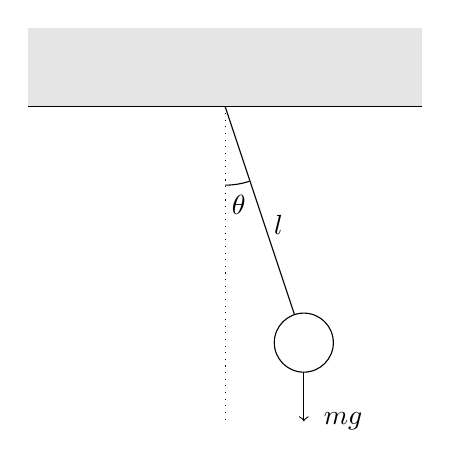
\begin{tikzpicture}[scale=0.5]
		\fill[color=gray!20] (-5,10) rectangle (5,8);
		\draw (0,6) arc (270:288:2);
		\node at (.35,5.5) {\(\theta\)};
		\draw (-5,8) -- (5,8);
		\draw (0, 8) -- node[right, midway]{\(l\)} (2, 2);
		\draw[dotted] (0, 8) -- (0, 0);
		\draw[->] (2,2) -- (2,0);
		\draw[fill=white] (2,2) ellipse (.75);
		\node at (3,0) {\(mg\)};
	\end{tikzpicture}
	\caption{Fuerzas que actúan sobre un péndulo}
	\label{fig:muelle}
\end{figure}

Recordamos que, por la segunda ley de Newton, \(F = ma\) donde \(a\) es la 
aceleración. Tenemos entonces que
\[-m g \sin\theta = m l \theta''\]
por tanto
\[\theta'' = -\frac{g}{l} \sin\theta\]
puesto que \(\theta\) aparece dentro del seno, esta ecuación es no lineal y de
orden 2, ya que aparece la derivada segunda de \(\theta\). En este caso
\(f(t, \theta, \theta') = -\frac{g}{l} \sin\theta\) y \(\Omega = \R \times
(-\pi, \pi) \times \R\). 

Si \(\theta\) es suficientemente próximo a \(0\) podemos aproximar 
\(\sin\theta\) a \(\theta\) con lo que tenemos la ecuación
lineal de segundo orden
\[\theta'' = -\frac{g}{l}\theta.\]

Esta es la ecuación del movimiento armónico simple. Su solución general, que,
recordamos, es el conjunto de todas las soluciones es
\[\theta(t) = C_1 \sin \omega t + C_2 \cos \omega t\]
donde \(\omega^2 = g/l\), demostraremos esto más adelante. Este conjunto de
soluciones forma un espacio vectorial de dimensión 2. Demostraremos también que
el conjunto de soluciones de una ecuación lineal de orden \(n\) es un espacio
vectorial, o afín si existe un término independiente, de orden \(n\).

\subsection{Problema de valor inicial (PVI)}

En los ejemplos anteriores hemos obtenido soluciones generales para los
problemas propuestos, pero si conocemos el valor de \(x\) y sus derivadas en un
tiempo determinado la solución de la ecuación diferencial está
unívocamente determinada, como demostraremos.

\begin{definition}[Problema de valor inicial]
	Un problema de valor inicial es una ecuación diferencial
	\[x^{(n)} = f(t, x, x', \dots, x^{(n - 1)}),\]
	junto a su valor y el de sus derivadas en un tiempo determinado \(t_0\)
	\[x(t_0) = x_0,\ x'(t_0) = x_1,\ \dots\ ,\ x^{(n - 1)}(t_0) = x_{n - 1}.\]
\end{definition}

\begin{definition}[Condición inicial]
	Llamaremos condición inicial al valor de \(x\) y sus derivadas en un tiempo
	determinado \(t_0\) en un problema de valor inicial.
\end{definition}

\subsection{Datación por radiocarbono}

Veremos como es posible datar un objeto conociendo solo la cantidad carbono 
presente en el mismo.

Existen diversos isótopos del carbono, entre ellos el carbono-12, el cual es
estable, y el carbono-14, el isótopo radiactivo más común. El carbono-14, al ser
radiactivo debería desintegrarse y disminuir su concentración en la atmósfera,
pero debido a los rayos cósmicos que constantemente alcanzan la tierra la
proporción entre estos dos isótopos se mantiene estable en la atmósfera. A
través de la fotosíntesis estos isótopos radiactivos pasan a formar parte de las
plantas y después, mediante la cadena alimenticia, del resto de seres vivos.
Cuando un ser vivo muere la cantidad de carbono-12 contenida en el mismo se
mantiene constante, mientras que la de carbono-14 disminuye anualmente,
a un ritmo que depende de su probabilidad de desintegración
\(\lambda \sim \log 2 / 5730\).

Con esto, analizando la proporción entre carbono-12 y 14 en
material orgánico (madera, hueso, etc.) y comparándolo con una muestra viva es 
posible determinar la edad del resto. La creación de este método de
datación valió al químico estadounidense Willard Libby el premio Nobel de
química en
1960\footnote{\url{https://es.wikipedia.org/wiki/Datación_por_radiocarbono}}.
Veamos algunos ejemplos concretos de como se puede aplicar esta
técnica.

\begin{example}
	Si la cantidad de carbono-14 en un microorganismo es de \(10^{-6}\) gramos
	¿Qué cantidad habrá 3000 años después?
\end{example}

\begin{solution}
	Se entiende que el ciclo de vida del organismo es despreciable respecto a la
	edad que debemos datar. Por lo visto arriba sabemos que \(x' = -\lambda x\).
	A tiempo \(0\), cuando el organismo muere, el valor de \(x\) es
	\(x(0) = 10^{-6}\). Se trata de un problema de valor inicial, que tendremos
	que resolver para poder encontrar \(x(3000)\). 

	Empezamos resolviendo la ecuación diferencial
	\[x(t) = k e^{-\lambda t} = k e^{-\frac{\log 2}{5730} t},\]
	por lo que hemos visto antes \(k = x(0) = 10^{-6}\) con lo que sin más que
	sustituir
	\[x(t) = 10^{-6} e^{-\frac{\log 2}{5730} t}.\]

	Podemos obtener ahora el resultado pedido 
	\(x(3000) = 6,95 \cdot 10^{-7}\) gramos.
\end{solution}

Normalmente no sabemos la cantidad total de carbono presente en un organismo
antes de su muerte, ni el tiempo transcurrido desde entonces. Veamos ahora un
ejemplo más cercano a la realidad.

\begin{example}
	En una excavación en Nippur, Babilonia, en 1950 el carbón vegetal de la viga
	de un techo dio \(4,09\) desintegraciones por minuto y gramo, mientras que
	la madera viva da \(6,68\) desintegraciones, también por minuto y gramo.
	Nos preguntamos en qué año se construyó en edificio.
\end{example}

\begin{solution}
	Llamaremos \(R(t)\) a la tasa de desintegración total
	\[R(t) = \lambda x(t) = \lambda x(0) e^{-\lambda t},\]
	donde \(x(0)\) es la
	cantidad de carbono-14 en el trozo de madera cuando fue cortada y \(t\) el
	tiempo transcurrido desde que se corta el árbol hasta 1950. Buscamos entonces
	el año de construcción, para ello observamos que \(R(0) = \lambda x(0)\), de
	donde el cociente \(\frac{R(t)}{R(0)} = e^{-\lambda t}\) no depende de la
	cantidad de carbono-14 presente en el organismo vivo \(x_0\). Sustituyendo
	los datos y despejando
	\[\frac{4,09}{6,68} = \frac{R(t)}{R(0)} = e^{-\frac{\log 2}{5730} t}
		\implies t \approx 4055,\]
	medido en años. Así, concluimos que el edificio se construyó en el \(2105\)
	a.C.
\end{solution}

\end{document}
